\chapter{Method of Approach} 
\label{ch:methodofapproach}

This section has been broken down into two parts that each detail how each of the main composer components were developed.  The first section describes the processes and tools needed to develop the composer and the second section describes the processes and ideas behind the development of the user interface.

\section{Computer Composer Development}
\label{sec:computercomposerdevelopment}

To begin this project, it was necessary to develop the composer which would function as the backend of the tool.  This was chosen as the first step because the elements of the user interface would have to be chosen and designed based on what the composer was capable of doing.  Without first implementing the basic functionalities of the composer, it would be impossible to determine how the user interface should be built.  To develop the functions of the composer, several preexisting python tools and libraries were employed.

\vspace{\baselineskip}

\subsection{Tools}
\label{subsec:tools}

The following table lists all of the tools that were used and their specific functions within the composer.  None of these tools, on their own, were capable of forming the functioning composer.  Several of these tools have very advanced sets of functions, but no single tool had all of the required functions for the composer.

\begin{table}[!htbp]
	\centering
	\caption{Tools and packages and their uses in this project}
	\begin{tabular}{|l|l|}
		\hline
		MusicXML Generation & music21 \\ \hline
		MIDI Generation & music21 \\ \hline
		Melodic Analysis & music21 \\ \hline
		Playback & MIDIjs \\ \hline
		Notation & OpenSheetMusicDisplay \\ \hline
	\end{tabular}
\end{table}

\subsubsection{music21}
\label{subsubsec:music21}

music21 is a Python tool for computer analysis of music and musical data \cite{Cuthbert_2020}.  It is capable of analysis of large and small works alike with analytical categories such as harmony, form, structure, pitch content, rhythmic content, lyric content, frequency, intervals, and counterpoint.  It is capable of performing roman numeral analysis and generating post-tonal matrices.  In this project, music21 is responsible for MusicXML generation, MIDI generation, and melodic analysis.

\vspace{\baselineskip}

music21 was chosen for this project due to its extensive analytical tools.  It is capable of powering all of the chosen elements of melodic analysis to assist the user during composition.  Several of the functions that are used within the feedback system are demonstrated below.

\vspace{\baselineskip}

This first example demonstrates how music21 is capable of checking for consonances and dissonances between pitches.  A starting and ending pitch are given and the function returns true if the interval is consonant and false if it is dissonant.  Intervals that are considered consonant by music21 are major or minor thirds or sixths, perfect fifths, unisons, and octaves.

\begin{figure}[!htbp]
	\caption{music21 Consonant Interval Checking \cite{Cuthbert_2020}}
	\code{> i1 = interval.Interval(note.Note(\textquotesingle C\textquotesingle ), note.Note(\textquotesingle E\textquotesingle ))} \\
	\code{> i1.isConsonant()} \\
	\code{True} \\
	\code{> i1 = interval.Interval(note.Note(\textquotesingle B-\textquotesingle ), note.Note(\textquotesingle C\textquotesingle ))} \\
	\code{> i1.isConsonant()} \\
	\code{False} \\
\end{figure}

This next example shows how music21 can identify the interval between two pitches.  The starting and ending notes are specified and a function is used to display the interval between them.  If \code{simpleName} is used, the interval is reduced to less than an octave.  If \code{semiSimpleName} is used, the interval is reduced to no more than an octave.

\begin{figure}[!htbp]
	\caption{music21 Interval Identification \cite{Cuthbert_2020}}
	\code{> n1 = note.Note(\textquotesingle c3\textquotesingle )} \\
	\code{> n2 = note.Note(\textquotesingle c5\textquotesingle )} \\
	\code{> aInterval = interval.Interval(noteStart=n1, noteEnd=n2)} \\
	\code{> aInterval.name} \\
	\code{\textquotesingle P15\textquotesingle } \\
	\code{> aInterval.simpleName} \\
	\code{\textquotesingle P1\textquotesingle } \\
	\code{> aInterval.semiSimpleName} \\
	\code{\textquotesingle P8\textquotesingle } \\
\end{figure}

This last example demonstrates how music21 can name a new pitch based on a starting pitch and an interval.  Once the starting pitch and the interval are given, a function can be used to return a new pitch based on a transposition of the first pitch.

\begin{figure}[!htbp]
	\caption{music21 Find Second Note Based on Interval \cite{Cuthbert_2020}}
	\code{> p1 = pitch.Pitch(\textquotesingle A\# 4\textquotesingle )} \\
	\code{> i = interval.Interval(\textquotesingle m3\textquotesingle )} \\
	\code{> p2 = i.transposePitch(p1)} \\
	\code{> p2} \\
	\code{<music21.pitch.Pitch C\# 5>} \\
\end{figure}

\subsubsection{MIDIjs}
\label{subsubsec:midijs}

MIDIjs is a JavaScript MIDI player that works with all modern browsers and is built entirely with JavaScript \cite{MIDIjs_ND}.  This tool was chosen for this project due to its high sound quality and ability to run without requiring any sort of download.  It runs in place and requires no plugins or extensions \cite{MIDIjs_ND}.  The following example shows how to play a MIDI file using MIDIjs.

\begin{figure}[!htbp]
	\caption{MIDIjs MIDI File Playback \cite{MIDIjs_ND}}
	\code{<script type=\textquotesingle text/javascript\textquotesingle  src=\textquotesingle //www.midijs.net/lib/midi.js\textquotesingle ></script>} \\
	\code{ <a href="\# " onClick="MIDIjs.play(\textquotesingle file.mid\textquotesingle );">Play file.mid</a>} \\
	\code{ <a href="\# " onClick="MIDIjs.stop();">Stop MIDI Playback</a>} \\
\end{figure}

\subsubsection{OpenSheetMusicDisplay}
\label{subsubsec:opensheetmusicdisplay}

OpenSheetMusicDisplay is web based tool that is capable of rendering MusicXML files into notation.  To use this tool, simply drag an XML file onto the webpage.  It will then render and display the file as music notation.  This tool was chosen due to its ease of use and for its ability to be used without having to perform any integration.

\subsection{Main Composer Process}
\label{subsec:maincomposerprocess}

The following diagram shows the composition process broken down into the specific actions of the computer and the user.  While the user is responsible for more actions than the computer, the user is assisted in the process by the specific design of the interface and the directions that are provided when using the composer.  The computer then assists the user with melodic analysis to verify the quality of the melody in practical music theory terms.

\begin{figure}[!htbp]
	\centering
	\caption{Composition Process Flowchart}
	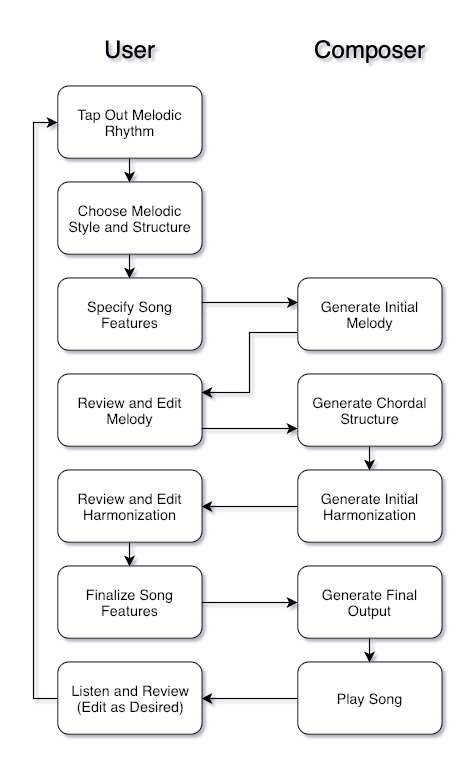
\includegraphics[scale=0.8]{images/composerProcess.png}
\end{figure}

\pagebreak

There are several important attributes that the user must choose when creating their melody.  The following table lists each of these elements and their definitions in the context of this tool.  It is important to note that none of these values are final and they can be changed at any time.

\begin{table}[!htbp]
	\centering
	\caption{Melody Initialization Attributes}
	\begin{tabular}{|l|l|}
		\hline
		Beats Per Minute & Number of base units per minute \\ \hline
		Base Beat & Base unit for time measurement and division \\ \hline
		Beats Per Bar & Number of base units in each measure of music \\ \hline
		Enharmonic Spelling & Determines if pitches are spelled as sharp or flat \\ \hline
		Pitch & Note name \\ \hline
		Duration & Length of time taken by a note \\ \hline
	\end{tabular}
\end{table}

\subsubsection{Beats Per Minute}
\label{subsubsec:beatsperminute}

In the context of this tool, tempo is represented as the number of beats that occur per minute.  This aligns with the standard definition of tempo as the rate at which beats pass.  The duration that defines the beat in this tool is what the user selected as the base note duration.

\subsubsection{Base Beat}
\label{subsubsec:basebeat}

In the context of this tool, this base note duration functions as the beat unit.  In music theory, the beat unit is defined as the note duration that gets the pulse.  This is the bottom number in a meter signature.  The user has the option to select 2, 4, 8, or 16 as the base duration.

\subsubsection{Beats Per Bar}
\label{subsubsec:beatsperbar}

To finish out the creation of the meter signature, the user must select the number of beats that will occur in each measure of music.  The user is not limited to any specific values here.  They can have as many or as few beats per bar as they desire.  In terms of the meter signature, this is the top number.

\subsubsection{Enharmonic Spelling}
\label{subsubsec:enharmonicspelling}

This option is used to change the default spelling of all of the pitches that contain sharps (\sh 's).  In the note input system, all of the pitches with accidentals are spelled with sharps.  This means that later, when the key is analyzed, the system would always return that the material is in a sharp-based key.  In order to provide access to flat-based keys as well, the user can specify that they want to spell these pitches with flats (\fl 's) instead of sharps by changing the enharmonic spelling option.

\subsubsection{Pitch}
\label{subsubsec:pitch}

Once this initial setup of the composition parameters is complete, the user can begin to enter the pitches and durations for each of the notes in the melody.  The user has access to all of the pitches from C3 to C6.  One octave of pitches is listed below with their enharmonic spelling (if applicable).  To select a pitch, the user checks one of 38 boxes that represent the 37 pitches in the allowed range and the rest option.

\begin{table}[!htbp]
	\centering
	\caption{Available Pitches and Enharmonic Equivalents}
	\begin{tabular}{|l|l|}
		\hline
		C & C \\ \hline
		C\sh & C\sh  or D\fl \\ \hline
		D & D \\ \hline
		D\sh & D\sh  or E\fl \\ \hline
		E & E \\ \hline
		F & F \\ \hline
		F\sh & F\sh  or G\fl \\ \hline
		G & G \\ \hline
		G\sh & G\sh  or A\fl \\ \hline
		A & A \\ \hline
		A\sh & A\sh  or B\fl \\ \hline
		B & B \\ \hline		
	\end{tabular}
\end{table}

\subsubsection{Duration}
\label{subsubsec:duration}

The musical durations and the representative decimal value that the user is able to choose from are listed in the following table.  The equivalent rest is available for each duration rest is selected instead of a pitch.  These values are based on a multiple of division of the value of a quarter note.  These are the values that music21 uses.

\begin{table}[!htbp]
	\centering
	\caption{Available Duration Values}
	\begin{tabular}{|l|l|l|}
		\hline
		Whole Note & \musWhole & 4 \\ \hline
		Dotted Half Note & \musHalfDotted & 3 \\ \hline
		Half Note & \musHalf & 2 \\ \hline
		Dotted Quarter Note & \musQuarterDotted & 1.5 \\ \hline
		Quarter Note & \musQuarter & 1 \\ \hline
		Dotted Eighth Note & \musEighthDotted & 0.75 \\ \hline
		Eighth Note & \musEighth & 0.5 \\ \hline
		Dotted Sixteenth Note & \musSixteenthDotted & 0.375 \\ \hline
		Sixteenth Note & \musSixteenth & 0.25 \\ \hline
	\end{tabular}
\end{table}

\subsubsection{Order}
\label{subsubsec:Order}

This property is included to easily allow the user to change the order of the notes in their composition.  The ideal use case is to give each new note a consecutive integer value (1, 2, 3, ...) and reserve the decimal places to insert notes between these notes when revising or editing.

\subsection{Notation and Playback}
\label{subsec:notationandplayback}

Once the user has entered some notes into their composition, they will be able to generate notation and playback of their melody.  The notes that are entered into the tool are parsed into a csv file that is then parsed into a music21 Stream.

\vspace{\baselineskip}

The Stream object has several conversion methods that are responsible for turning it into a MusicXML file and a MIDI file.  The MIDI file is passed off to MIDIjs for playback and the MusicXML file is passed to OpenSheetMusicDisplay to display the notation.

\subsection{Melodic Analysis}
\label{subsec:melodicanalysis}

It is during this part of the process that the system generates feedback on the user's melody and provides suggestions for how to improve it.  The following list details each of the areas of feedback and the specific functions within music21 that will handle the checks.  These rules for "good" melodies are based in western music.  By referring to these rules as "what makes a good melody" it is simply to say that these are some of the properties of melodies in western music that have proven to make melodies that are pleasing to hear and easy to perform.  This is not to say that melodies that do not follow these rules are bad.  These are just some guidelines to help those that are new to melody creation.

\begin{itemize}
	\item Range
	\begin{itemize}
		\item Typically, the range from the lowest note to the highest note should be under an octave and a half.  This is to make sure that the melody is within a range that most people and instruments can produce good sound. \\ \\
		\code{> analysis.discrete.Ambitus().getPitchSpan(input)} \\
		\item This function returns the difference between the lowest and highest note by calculating the pitch space.  Conditional statements are then used to determine if this is within the appropriate range.
	\end{itemize}
	\item Contour
	\begin{itemize}
		\item The melody should consist mostly of stepwise motion.  This means that there should be primarily movement by whole and half steps (conjunct motion) with some leaps (disjunct motion) added for interest.  Generally, leaps should be used to outline a climax in the phrase and work towards the resolution with stepwise motion.  It is also a good idea to keep the size of the leap no more than an octave. \\ \\
		\code{> voiceLeading.NNoteLinearSegment(listOfNotes).melodicIntervals} \\
		\item This function returns a list of the intervals between each consecutive note in the melody.  An iterator counts the number of conjunct and disjunct movements and generates a recommendation if the ratio of steps to leaps is less than 3:1.  If an interval is found to be greater than an octave, an additional recommendation is generated.
	\end{itemize}
	\item Intervals
	\begin{itemize}
		\item When melodies do contain leaps, these leaps should be of consonant rather than dissonant intervals.  Consonant leaps include major or minor thirds or sixths, octaves, perfect fifths, and, in the case of more modern music, perfect fourths.  Following a leap, the melody should move in stepwise motion in the opposite direction as the leap.  Dissonant leaps include major or minor sevenths and tritones. \\ \\
		\code{> interval.Interval(note1, note2).isConsonant()} \\
		\code{> interval.Interval(noteStart=note1, noteEnd=note2).name} \\
		\code{> interval.Interval(noteStart=note1, noteEnd=note2).semiSimpleName} \\
		\item The first of these functions will flag particular intervals as dissonant and then these will be saved to a list.  These particular intervals are then identified and displayed to the user using the next two functions.
	\end{itemize}
	\item Key Relation
	\begin{itemize}
		\item Typically, the majority of the material in a melody should belong to a particular key.  If the key is E\fl Major, one should see E\fl , F, G, A\fl , B\fl , C, and D.  If there are lots of F\sh 's, then it is most likely not E\fl Major.  \\ \\
		\code{> stream.analyze(\textquotesingle key\textquotesingle)} \\
		\code{> stream.analyze(\textquotesingle key\textquotesingle).correlationCoefficient} \\
		\item Using these methods, it is possible to determine the key and to determine how close the pitch content of the melody is to that key.  The closer to one the value is, the closer it is to the analyzed key.  The closer to zero the value is, the farther it is from that key.
	\end{itemize}
\end{itemize}

\subsection{Melody Feedback}
\label{subsec:melodyfeedback}

Based on the areas of melodic development that are listed above, the tool will generate feedback to the user about what they could improve.  It is possible to disregard all of the feedback and proceed with finalizing the melody.  The feedback is there as a suggestion for those that may not know how to compose a melody or someone who is struggling to write a melody that they are pleased with how it sounds.  It is not required to use any of the feedback.

\vspace{\baselineskip}

That being said, once the feedback is presented, the user will be able to continue to make changes and reanalyze their melody.  The feedback will reflect whatever changes they make.  It is also the case that a user may choose to follow certain suggestions and not others.  This is totally acceptable as the feedback is meant to help, but not to hinder creativity.

\vspace{\baselineskip}

If the user is presented with feedback in terms of range, the tool will point out what exactly is out of range and suggest that the user alter these notes or move them up or down an octave.  If the user is given feedback about contour, the tool will show which specific leaps and following notes need to be addressed.  If there is an issue with the ratio of conjunct to disjunct movements it will highlight the leaps and make suggestions about how to alter them.

\vspace{\baselineskip}

If the user receives feedback related to the intervals within their melody, the tool will address the specific intervals that violate the given rules and use the transposition feature, that was highlighted earlier, to present alternative pitch options to correct the error.  Additionally following each leap, the system will check to see if there is stepwise resolution using the same functions as the contour checking system.  If this is not present, the system will recommend that the user add it and show them how.  If the user gets feedback on their resolution of the melody, the system will recommend alternate notes based on the key they have chosen.

\subsection{Output}
\label{subsec:output}

There are several stages of transformation that the data within the composer undergoes by the time that it reaches the end of the process.

\subsubsection{Composer}
\label{subsubsec:composer}

The output from the composer is a SQLite database with all of the composition and note objects stored within it.  The following images are screenshots of a database viewing tool to show what the composition and note tables look like after entering values into the UI.

\begin{figure}[!htbp]
	\centering
	\caption{Database Composition Table}
	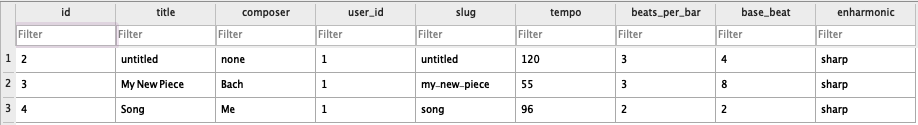
\includegraphics[scale=0.45]{images/compositionTable.png}
\end{figure}

\begin{figure}[!htbp]
	\centering
	\caption{Database Note Table}
	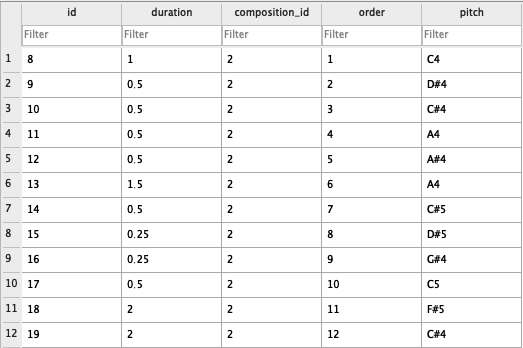
\includegraphics[scale=0.45]{images/noteTable.png}
\end{figure}

\subsubsection{Parsing}
\label{subsubsec:parsing}

At this step in the output process, a Python program reads the database and saves the values into CSV files by the composition id.  The following images show the contents of the composition and notes CSV files.

\begin{figure}[!htbp]
	\centering
	\caption{Composition CSV}
	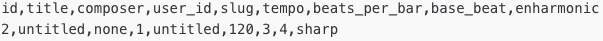
\includegraphics[scale=0.7]{images/compositionCSV.png}
\end{figure}

\begin{figure}[!htbp]
	\centering
	\caption{Notes CSV}
	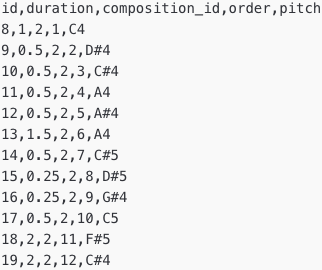
\includegraphics[scale=0.7]{images/notesCSV.png}
\end{figure}

\subsubsection{music21}
\label{subsubsec:outputmusic21}

Once the CSV files are generated, music21 reads the data from these files and builds this into a Stream object.  If you were to call a print function on the Stream, it would appear as the following:

\begin{figure}[!htbp]
	\centering
	\caption{Note Stream}
	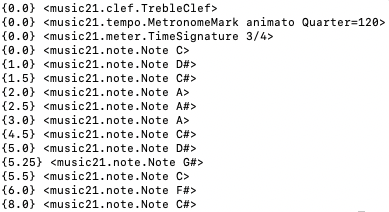
\includegraphics[scale=0.7]{images/noteStream.png}
\end{figure}

\subsubsection{Files}
\label{subsubsec:files}

The Stream is converted by music21 into an XML file and a MIDI file.  The XML file can be dropped into OpenSheetMusicDisplay to see the notation.  There is a playback button within the UI that takes the MIDI file and passes it to MIDIjs.  An example of the notation is displayed below.

\begin{figure}[!htbp]
	\centering
	\caption{Notation Output}
	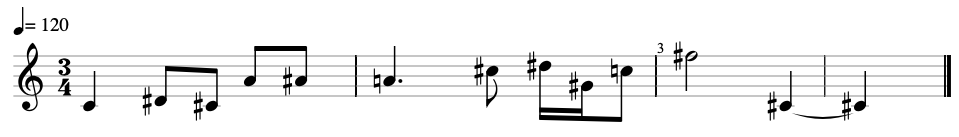
\includegraphics[scale=0.4]{images/notation.png}
\end{figure}

\section{User Interface Development}
\label{sec:userinterfacedevelopment}

The next phase of this project was to develop the user interface.  While there were a number of challenges that have prevented full integration of the tool with the interface, the interface does work and is available to use for a number of functions.

\subsection{Methodology}
\label{subsec:methodology}

This section details the background thinking and ideas that went into creating the user interface.

\subsubsection{Design}
\label{subsubsec:methodologydesign}

It is a common debate in interface design (and design in general) whether form should follow function or vice versa.  In the case of this project, it is necessary that the design of a particular element should reveal its function.  The user should be able to look at a particular button or slider, and without much effort, be able to figure out what it does.

\vspace{\baselineskip}

Due the varying levels of music or computer science knowledge elements of the UI needed to be designed in a way that is simple and clear.  There cannot be huge numbers of controls and there also cannot be any assumptions as to what a particular thing should do.  The design of a component needs to spell out what it does.

\subsubsection{Functions}
\label{subsubsec:methodologyfunctions}

When thinking about the functions of the interface it must: 1) provide access to the initial setup parameters; 2) display the note input system; 3) provide instructions for use; 4) provide access to the feedback system; 5) display the notation and playback window.  Each of these functions are required in order to be able to fully interact with the composer.

\vspace{\baselineskip}

Additionally, the access to these functions must be direct.  The user must specifically be able to call each of these functions and see their output.  There are other internal functions of the system, but these are not made to be accessible through the interface.

\subsubsection{Layout}
\label{subsubsec:methodologylayout}

Due to the detail required in the note input system, the layout of the UI has been optimized for desktop browsers.  While it is possible to view and use the site on mobile, it is not recommended.  The design of the note input system, in its current form, cannot be made small enough to be usable on a mobile device.

\vspace{\baselineskip}

To make the tool easier to use, everything must be large enough and have adequate space in between.  This is to prevent misclicks and errors when entering notes and accessing other functions.

\subsection{Process}
\label{subsec:process}

This section details the tools and processes that were used in the creation of the user interface.

\subsubsection{Design}
\label{subsubsec:processdesign}

The design of the user interface was done primarily with Bootstrap Studio under the free education license.  Bootstrap was chosen for this project to allow for a flexible layout of the controls and UI elements.  Bootstrap Studio was chosen specifically for its graphical design interface to speed up the process of building in individual items.

\vspace{\baselineskip}

When exporting a design from Bootstrap Studio, it includes the Bootstrap files, CSS, JavaScript, and HTML.  There was some adaptation required to mesh these designs with the backend of the tool, but this process was fairly straightforward.

\vspace{\baselineskip}

Once the general layout was complete, additional tweaks and adjustments were made to each page based on how it had to interact with the backend of the tool.  The specifics of this are discussed in the layout section.

\subsubsection{Functions}
\label{subsubsec:processfunctions}

To power the UI and the backend of the tool, this project uses Django.  This is a Python based web framework that allows for the integration of a database and custom Python functions with a HTML based interface.

\vspace{\baselineskip}

This tool was chosen for its project due to its high level of customization, user authentication system, integration with a database, and UI design tools.  For this tool, the database is written in SQLite.  This keeps the integration with Django simple as this is the default option.

\vspace{\baselineskip}

Within Django, custom models for the user, composition, and note objects were created.  The notes are linked to the composition by foreign key and the compositions are linked to the user by foreign key.  This means that users only have access to their compositions and each composition only has access to its notes.

\vspace{\baselineskip}

The composition model contains all of the fields that are part of the initial setup of the composition (title, composer, tempo, base beat, beats per bar, and enharmonic).  The composition model also contains an id, slug, and user field. 

\vspace{\baselineskip}

The id is unique for each composition and is used to attach each note to its composition.  The slug is what allows for the viewing and editing of each composition.  This value is generated by a unique function to ensure that no two compositions have the same slug.  The slug is what is passed into the URL to locate a particular composition.  The user field is what gives ownership of a particular composition to the user that created it.  This way, users cannot edit each other's compositions.

\vspace{\baselineskip}

The note model contains the fields necessary for music21 to be able to create a note (pitch and duration) and fields that allow Django to be able to find and display the note (id, composition, and order).

\vspace{\baselineskip}

The pitch field allows the user to select from any pitch between C3 and C6 as mentioned above.  The choices are hard-coded so that the user simply has to select one without needing to type the value in.  The duration field is the same in this regard.  The available values are the ones that were listed above.

\vspace{\baselineskip}

The id for the note functions the same was as the id for the composition.  The composition field is what links the note to a particular composition.  This value is automatically filled when a note is created.  The order property determines the order that Django should return the list of notes.

\subsubsection{Layout}
\label{subsubsec:processlayout}

The note input controls were developed to resemble a piano, but knowledge of the keyboard is not required to enter notes.  It is labeled like a keyboard to provide some representation of what the actual pitches are.  Without this, there would be no way to distinguish notes from each other (other than that a different note is either higher or lower on the list of boxes).

\vspace{\baselineskip}

The initial input radio buttons are displayed for each available pitch and the rest.  After the note is entered, the buttons are replaced by the image of the keyboard with a darkened version of whatever pitch was selected and the set of buttons moves over.  This continues for each note that is added.

\vspace{\baselineskip}

Below, is an image of the note boxes for the example composition that was presented in the output section.

\begin{figure}[!htbp]
	\centering
	\caption{Note Boxes with C4 Selected}
	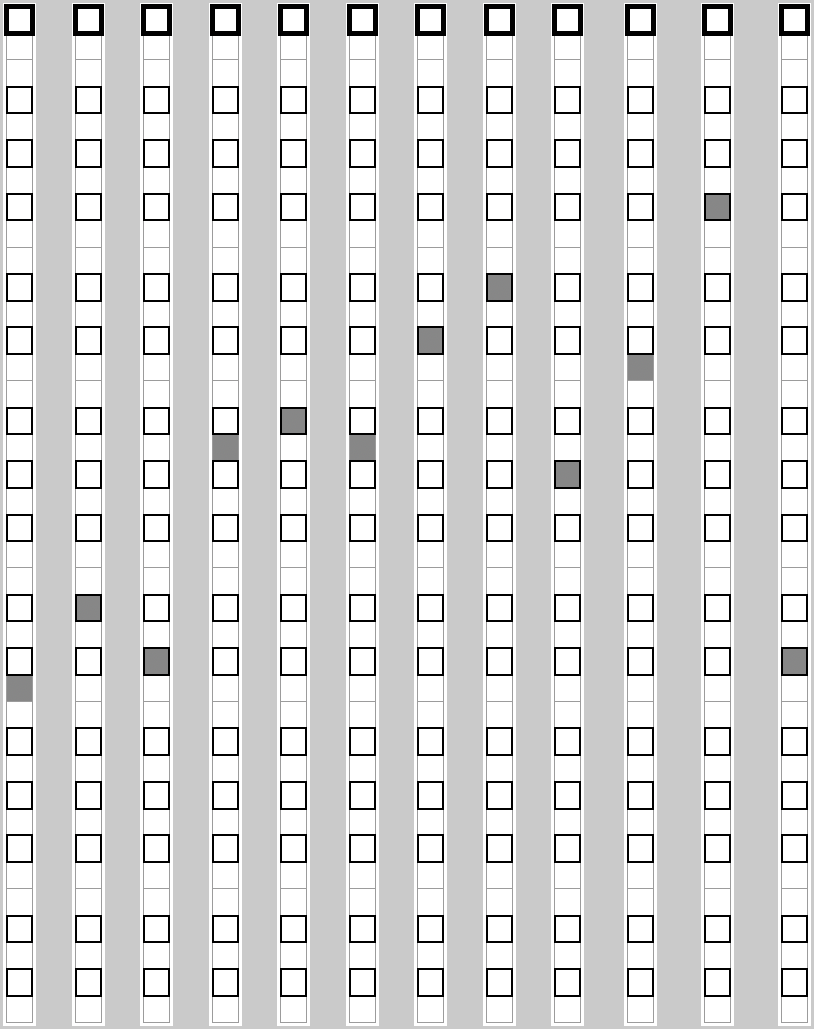
\includegraphics[scale=0.45]{images/noteBoxes.png}
\end{figure}